\section{Inference}

Now that we have defined the LBGM, we wish to leverage it to perform inference. Suppose we are presented with a vertex-labelled graph $(A, X)$; the goal is to draw samples for $\theta$ according to the posterior given the observed graph (equation \ref{eqn:theta-target}). 
%
\begin{equation}
	\label{eqn:theta-target}
	\theta^{(t)} \sim p(\theta | A, X)
\end{equation}
%
These samples allow us to approximate the posterior distribution for $\theta$ as well as compute a predictive distribution $p(b^* | x^*, A, X) = \int p(b^* | x^*, \theta) p(\theta | X, A) d\theta \approx \frac{1}{T} \sum_{t=1}^{T} p(b^* | x^*, \theta^{(t)})$. However, generating these samples is not easily done in practice.

We instead propose an iterative approach. First drawing samples $b^{(t)}$ from the block membership posterior (equation \ref{eqn:b-samples}). We then use each $b^{(i)}$ to draw samples for $\theta$ as in equation \ref{eqn:theta-samples}. 
%
\begin{align}
	b^{(i)} &\sim p \Big( b | A, X \Big)  \label{eqn:b-samples}\\
	\theta^{(i)} &\sim p\Big(\theta | X, b^{(i)} \Big) \label{eqn:theta-samples}
\end{align}
%
Both of these sampling steps implemented with a Markov Chain through the Metropolis-Hastings algorithm \cite{hastings-alg}. We just need to define a proposal distribution $q(x, x')$ for proposing a move $x \rightarrow x'$ and be able to evaluate an un-normalised form of the target distribution, denoted $\pi(\cdot)$, point-wise. The proposed move is then accepted with probability $\alpha$ (equation \ref{eqn:mh-accept}) else it is rejected and we stay at $x$.
%
\begin{equation}
	\alpha = \min \left( \frac{\pi(x') q(x', x)}{\pi(x) q(x, x')} , 1 \right)
	\label{eqn:mh-accept}
\end{equation}
%
This accept-reject step ensures the resulting Markov Chain is in detailed balance with the target distribution $\pi(\cdot)$. What we propose in equations \ref{eqn:b-samples} and \ref{eqn:theta-samples} is therefore implemented through a 2-level Markov chain. The resulting samples for $\theta^{(i)}$ are unbiased in the sense that the expectation of their distribution is the posterior we are targeting in equation \ref{eqn:theta-target}.
%
\begin{align*}
	\Expect_{b^{(t)}} \left[p \left( \theta | X, b^{(t)} \right) \right] &= \sum_{b \in \mathcal{B}^N} p(\theta | X, b) p(b | A, X) \\
	&= \sum_{b \in \mathcal{B}^N} p(\theta, b | A, X) \\
	&= p(\theta | A, X) \\
\end{align*}
%
This is an example of a pseudo-marginal approach \cite{pseudo-marginal}. Indeed, the unbiased result is sufficient to prove that for sufficient samples, $\theta^{(t)} \sim \Expect_{b^{(i)}} \left[ p(\theta | X, b^{t})\right] = p(\theta 
\ A, X)$ which is exactly the distribution we were targetting (equation \ref{eqn:theta-target}).

The reason we split the Markov chain into two stages is because the summation over all latent states $b \in \mathcal{B}^N$ required to directly compute the likelihood $p(A| X, \theta) = \sum_{b \in \Bcal^N} p(A | b) P(b | X, \theta)$ is intractable $O(B^N)$.
%
\begin{figure}[!h]
	\centering
	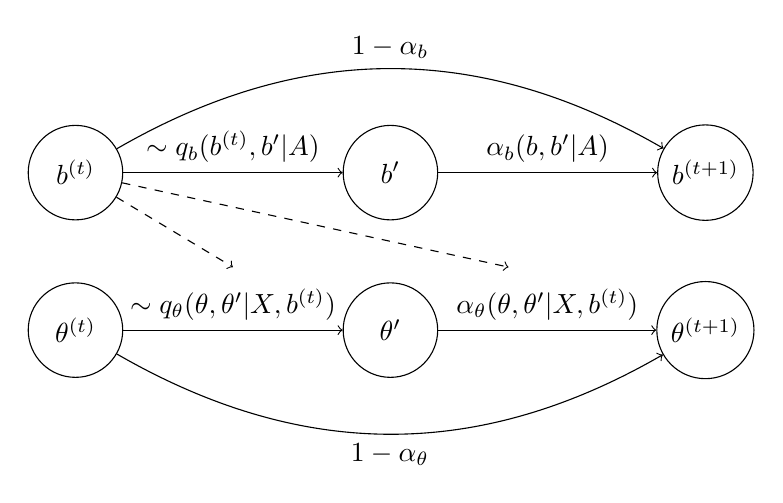
\begin{tikzpicture}[
		roundnode/.style={circle, draw=black, minimum size=12mm},
		squarednode/.style={rectangle, draw=black, minimum size=12mm}
		]
		% nodes
		\node[roundnode] (b0) at (0, 2) {$b^{(t)}$};
		\node[roundnode] (b1) at (4, 2) {$b'$};
		\node[roundnode] (b2) at (8, 2) {$b^{(t+1)}$};
		\node[roundnode] (t0) at (0, 0) {$\theta^{(t)}$};
		\node[roundnode] (t1) at (4, 0) {$\theta'$};
		\node[roundnode] (t2) at (8, 0) {$\theta^{(t+1)}$};
		
		% arrows
		\draw[->] (b0) to node[above] {$\sim q_b(b^{(t)}, b' | A)$} (b1);
		\draw[->] (b1) to node[above] {$\alpha_b (b, b' | A)$} (b2);
		\draw[->] (b0) [out=30, in=150] to node[above] {$1-\alpha_b$} (b2);
		
		\draw[->] (t0) to node[above] {$\sim q_\theta(\theta, \theta' | X, b^{(t)})$} (t1);
		\draw[->] (t1) to node[above] {$\alpha_\theta (\theta, \theta' | X, b^{(t)})$} (t2);
		\draw[->] (t0) [out=-30, in=-150] to node[below] {$1-\alpha_\theta$} (t2);
		
		\draw[dashed, ->] (b0) to (2, 0.8);
		\draw[dashed, ->] (b0) to (5.5, 0.8);
		
	\end{tikzpicture}
	\caption{Sampling sequence}
	\label{fig:samp-sequence}
\end{figure}
%
Figure \ref{fig:samp-sequence} shows an overview of the proposed method. We have introduced subscripts and conditionings to make explicit what parameters each step utilises. In an important simplification, we note that $p(b| X) = B^{-N}$ which does not depend on the exact value of X. Therefore, we do not need to know the value of $X$ to perform the sampling on $b$. Conversely, for the $\theta^{(t)}$ samples, we use $b^{(t)}$ but not $A$ as $(\theta \indep A) | b$.

\subsection{Sampling block memberships}

\citet{Peixoto-MCMC} proposes a Monte Carlo method which we will base our approach on. It relies on writing the posterior in the following form:
%
\begin{equation}
	p(b | A, X) \propto p(A | b, X) \cdot p(b | X) = \pi_b(b)
\end{equation}
%
Now $\pi_b(\cdot)$ is the un-normalised density we wish to sample from. In other words, we wish to construct a Markov chain that has $\pi_b(\cdot)$ as its invariant distribution. We can break $\pi_b$ down as follows:
%
\begin{align*}
	\pi_b(b) &= p(b|X) \sum_{\psi} \nolimits p(A , \psi | b, X) \\
	&= p(b|X) p(A, \psi^* | b, X) \\
	&= p(A | b, \psi^*) \cdot p(\psi^* | b) \cdot p(b | X)
\end{align*}
%
Since we are using the microcanonical SBM formulation, there is only one value of $\psi$ that is compatible with the given $(A, b)$ pair. We denote this value $\psi^* = \{k^*, e^*\}$. Specifically, $k^*_i = \sum_j A_{ij} $ and $e^*_{rs} = \sum_{i, j} A_{ij} \one \{b_i=r\} \one\{b_j=s\}$. Therefore, the summation over all $\psi$ reduces to just the single $\psi^*$ term. We also define the microcanonical entropy of the configuration as.
%
\begin{equation}
	S(b) = - \log \pi_b(b) = - \Big( \log p(A | b, \psi^*) + \log p(\psi^*, b | X) \Big)
\end{equation}
%
This entropy can be thought of as the description length of the graph because it is the sum of the information required to represent the graph given the parameters and the amount of information required to store the parameters (given the feature matrix $X$). The exact, from of the proposal distribution and accept-reject step is explored throughly by \citet{Peixoto-MCMC}. There is a widely used library for Python made available under LGPL called \verb*|graph-tool| \cite{peixoto_graph-tool_2014}, which implements this algorithm. The only modification we make is in the block membership prior $p(b)$ which we replace with $p(b|X)=B^{-N}$ which is a uniform distribution and so cancels out in the MH accept-reject step.

The end result of this is that we can generate a set of block membership samples $\{b^{(t)}\}_{t=1}^{T}$ with each $b^{(t)} \sim p(b | A, X)$. Each of these samples can then be used for the $\theta$-chain.

\subsection{Sampling feature-to-block classifier parameters}

The invariant distribution we wish to target for the $\theta$ samples is the posterior of $\theta$ given the values of the pair $(X, b)$. We write this as follows:
%
\begin{align}
	p(\theta | X, b) &\propto p(b | X, \theta) p(\theta) = \pi_\theta (\theta) \propto  \exp \left( - U(\theta) \right) \\
	\therefore U(\theta) &= - \left( \log p(b | X, \theta) + \log p(\theta) \right) + \textrm{const}
\end{align}
%
Where we have introduced $U(\theta)$ equal to the negative log posterior. This $U(\theta)$ term makes subsequent analysis more concise. Each of the constituent terms of $U(\theta)$ is easily computed (equation \ref{eqn:U-constituent-terms}). To simplify notation, we define $y_{ij} \coloneqq \one \left\{ b_i = j \right\}$ and $a_{ij} \coloneqq \phi_j(x_i; \theta)$.
%
\begin{equation}
	\log p(b | X, \theta) = \sum_{i=1}^{N} \sum_{j=1}^{B} y_{ij} \log a_{ij}  \quad \textrm{and} \quad
	\log p(\theta) = -\frac{(D+1)(B)}{2} \log 2\pi - \frac{1}{2 \sigma_\theta^2} || \theta ||^2
	\label{eqn:U-constituent-terms}
\end{equation}
%
This means that if we ignore constant terms we can write $U(\theta)$ as in equation \ref{eqn:U-form}. We see that the prior effectively introduces a regularisation term. Note that $||\theta||^2 = \sum_{i} \theta_{i}^2 = \sum_{j=1}^{B} ||w_j||^2$ is the Euclidean norm of the vector of parameters $\theta$.
%
\begin{equation}
	U(\theta) = \left( \sum_{i=1}^{N} \sum_{j=1}^{B} y_{ij} \log \frac{1}{a_{ij}} \right)
	+ \frac{1}{2\sigma_\theta^2} ||\theta||^2
	\label{eqn:U-form}
\end{equation}
%
$U(\theta)$ in equation \ref{eqn:U-form} appears a typical objective function to be minimised for neural network training. The first term is the cross-entropy between actual and predicted labels. The second term - introduced by the prior - brings a form of regularisation, preventing over-fitting. In traditional applications we only seek the value of $\theta$ that minimises the objective function $U(\theta)$, which in our case would yield the maximum a posteriori (MAP) estimate. This is often done through some kind of gradient descent as $\nabla U$ is easily computable (equation \ref{eqn:U-derivative}).

However, our goal is not to find the MAP estimate but to draw samples from the posterior $\pi_\theta(\cdot) \propto \exp(-U(\cdot))$. As discussed earlier, given the invariant $\pi_\theta(\cdot)$, it is sufficient to specify a proposal distribution and then apply a MH accept-reject step to ensure detailed balance of the Markov Chain. Nevertheless, we can use $\nabla U$ as a useful heuristic to bias our proposal towards regions of higher target density. We therefore adopt the Metropolis Adjusted Langevin Algorithm (MALA) - first proposed by \citet{mala-tweedie} - which leverages just that. Given the current sample $\theta$, we propose a new sample $\theta'$ according to equation \ref{eqn:theta-update}
%
\begin{equation}
	\theta' = \theta - h \nabla U(\theta) + \sqrt{2h} \cdot \xi
	\label{eqn:theta-update}
\end{equation}
%
Where $\xi \sim \Gaussian(0, I)$ and $h$ is a step-size parameter - which may vary with the sample index. Indeed without the injected noise term, this is equivalent to gradient descent. We require the noise term to fully explore the parameter space. As such the proposal distribution, is a simple multivariate Gaussian which can be easily evaluated.
%
\begin{equation}
	q_\theta(\theta, \theta') = \Gaussian \left( \theta' ; \theta - h \nabla U(\theta), 2h I \right)
\end{equation}
%
The term $\nabla U$ has an easy to compute analytic form (derived in Appendix \ref{appdx:gradu}). By noting that $\theta = \{w_k\}_{k=1}^{B}$, we write the derivative with respect to each $w_k$ as:
%
\begin{equation}
	\frac{\partial U}{\partial w_k} = - \left( \sum_{i=1}^{N} \Big\{ \tilde{x}_i (y_{ik} - a_{ik}) \Big\} - \frac{w_k}{\sigma_\theta^2} \right)
	\label{eqn:U-derivative}
\end{equation}
%
After a proposed move is generated, in typical Metropolis-Hastings fashion we accept the move with probability $\alpha_\theta$.
%
\begin{equation}
	\alpha_\theta(\theta, \theta') = \min \left( 
	\exp \left( U(\theta) - U(\theta')\right)
	\frac{ 
		q_\theta(\theta', \theta)
	}{
		q_\theta(\theta, \theta')
	} 
	, 1 \right)
\end{equation}
%
This fully specifies, the sampling procedure to generate $\{\theta^{(t)}\}_{t=1}^T$. Bear in mind that each $\theta^{(t)}$ update step uses its corresponding $b^{(t)}$ block membership sample.

\subsection{Sampling sequence}

So far, each $\theta^{(t)}$ update uses its corresponding $b^{(t)}$ sample. This means that the evaluation of $U(\theta)$ and $\nabla U(\theta)$ has high variance. This may lead to longer burn-in and autocorrelation times of the resulting Markov Chain. The only link between $b^{(t)}$ and $\theta^{(t)}$ is in the evaluation of $U(\theta)$ and $\nabla U(\theta)$ which depends on $y_{ij}^{(t)} \coloneqq \one\{b_i^{(t)} = j\}$. We would rather deal with the expectation of each $y_{ij}^{(t)}$:
%
\begin{equation}
	\Expect \left[ y_{ij}^{(t)} \right] = \Expect_{b^{(t)}} \left[ \one(b_{i}^{(t)} = j) \right]
	= p(b_i = j | A, X)
\end{equation}
%
We obtain an unbiased estimate for this quantity as simply the empirical distribution of the block membership samples $\left\{ b^{(t)} \right\}_{t=1}^T$.
%
\begin{equation}
	\hat{y}_{ij} \coloneqq \frac{1}{T} \sum_{t=1}^{T} y_{ij}^{(t)} = \frac{1}{T} \sum_{t=1}^{T} \one\{b_i^{(t)} = j\}
\end{equation}
%
We therefore, choose to feed each $\theta^{(t)}$ update step the same $\hat{y}_{ij}$ for all $t$ rather than the corresponding $y^{(t)}_{ij}$. This means we no longer need to run the $b$ and $\theta$ Markov chains concurrently. Instead, we run the $b$-chain to completion and use it to generate $\hat{y}_{ij}$ for $i \in \{1 \dots N\}$ and $j \in \{1 \dots B\}$. This is an estimate of $p(b | A, X)$ that we use for every iteration of the $\theta$ Markov chain. This affords us the flexibility to vary the number of samples we draw for $b$ and $\theta$; wed refer to these as $T_b$ and $T_\theta$ henceforth. Furthermore, this changeover reduces the burn-in time for the $\theta$-chain by reducing the variance in our evaluation of $U$ and $\nabla U$.

\begin{algorithm} % enter the algorithm environment
	\caption{Block membership sample generation} % give the algorithm a caption
	\label{alg:b-samples} % and a label for \ref{} commands later in the document
	\begin{algorithmic} % enter the algorithmic environment
		
		\FOR{$t \in \{0, 1 \dots T_b - 1\}$}
		\STATE $b' \gets \sim q_b(b^{(t)}, b' | A)$
		\STATE $\log \alpha_b \gets \log \alpha_b(b^{(t)}, b' | A)$
		\STATE $\eta \gets \sim \textrm{Unif}(0,1)$
		\IF{$\log \eta < \log \alpha_b$}
		\STATE $b^{(t+1)} \gets b'$
		\ELSE
		\STATE $b^{(t+1)} \gets b^{(t)}$
		\ENDIF
		\ENDFOR
		
		\STATE \textbf{return} $\{b^{(t)}\}_{t=1}^{T_b}$
		
	\end{algorithmic}
\end{algorithm}

\begin{algorithm} % enter the algorithm environment
	\caption{LBGM parameter pseudo-marginal inference} % give the algorithm a caption
	\label{alg:theta-samples} % and a label for \ref{} commands later in the document
	\begin{algorithmic} % enter the algorithmic environment
		
		\STATE $\mathcal{S} \gets \textrm{range}(\textrm{burn-in}, T_b, \textrm{thinning})$
		\STATE $\hat{Y}_{ij} \gets \frac{1}{\mathcal{|S|}} \sum_{t \in \mathcal{S}} \one \{ b^{(t)}_i = j\} \quad \forall i,j$
		
		\item[]
		
		\FOR{$t \in \{0, 1 \dots T_\theta - 1\}$}
		\STATE $\xi \gets \sim \Gaussian(0, I)$
		\STATE $\theta' \gets \theta^{(t)} - h_t \nabla U(\theta^{(t)} | X, \hat{Y}) + \sqrt{2h_t} \cdot \xi$
		\STATE $\log \alpha_\theta \gets \log \alpha_\theta(\theta^{(t)}, \theta' | A, \hat{Y})$
		\STATE $\eta \gets \sim \textrm{Unif}(0,1)$
		\IF{$\log \eta < \log \alpha_\theta$}
		\STATE $\theta^{(t+1)} \gets \theta'$
		\ELSE
		\STATE $\theta^{(t+1)} \gets \theta^{(t)}$
		\ENDIF
		\ENDFOR
		
		\STATE \textbf{return} $\{\theta^{(t)}\}_{t=1}^{T_\theta}$
		
	\end{algorithmic}
\end{algorithm}

\subsection{Complexity Analysis}

\subsection{Choosing the number of blocks}

For the purposes of our model (the LBGM), the number of blocks $B$ is a constant which must be specified by the data scientist. We could however, allow our choice of $B$ to be influenced by the observed data. This places us in the domain of empirical Bayes, which must be negotiated carefully. Prior beliefs must be determined a priori else they are not prior. However, as the number of blocks only specifies the coarseness of the analysis, it is fine to allow it to vary. Indeed, \citet{peixoto-determine-B} shows that for a fixed average degree the maximum number of detectable blocks scales as $O(\sqrt{N})$ where $N$ is the number of vertices.

If we allow $B$ to vary in the $b$-chain (i.e. new blocks can be created and we permit empty blocks) then it can be run  until a minimum description length (MDL) solution is reached. We take the number of non-empty blocks at the MDL to be our fixed block number $B$ for subsequent analysis. Indeed, it is prudent to start our $b$-chain at this MDL solution as then the burn-in time is greatly reduced.